\documentclass{beamer}
\usepackage{graphicx} % Allows including images
\usepackage{booktabs} % Allows the use of \toprule, \midrule and \bottomrule in tables
\usepackage{amsmath}
\usepackage{epstopdf}
\usepackage{dsfont}

\DeclareMathOperator{\probability}{Pr}
\DeclareMathOperator*{\argmax}{arg\,max}
\DeclareMathOperator*{\argmin}{arg\,min}


\usetheme{Warsaw}
%\usetheme{Copenhagen}

\title{Chapter 2: Classifications of systems}
%\subtitle{A Library for Ensemble Learning Using Support Vector Machines}
\author{}
%\institute{KU Leuven}
%\institute{ESAT-STADIUS, KU~Leuven \\ iMinds Medical IT Department}

\definecolor{blueish}{rgb}{0.3,0.3,0.7}

\AtBeginSection[]
{
\begin{frame}<beamer>
\frametitle{Outline}
\tableofcontents[currentsection]
\end{frame}
}

\AtBeginSubsection[]
{
\begin{frame}<beamer>
\frametitle{Outline}
\tableofcontents[currentsubsection]
\end{frame}
}

\newif\ifpdf
\ifx\pdfoutput\undefined
\pdffalse
\else
\pdfoutput=1
\pdftrue
\fi
\ifpdf
%nessim
\epstopdfsetup{suffix=}
\DeclareGraphicsRule{.eps}{pdf}{.pdf}{`epstopdf #1}
\pdfcompresslevel=9
\else
\usepackage{graphicx}
\fi

\begin{document}

\begin{frame}
\titlepage % Print the title page as the first slide
\end{frame}

\begin{frame}
\frametitle{Overview} % Table of contents slide, comment this block out to remove it
\tableofcontents % Throughout your presentation, if you choose to use \section{} and \subsection{} commands, these will automatically be printed on this slide as an overview of your presentation
\end{frame}

%----------------------------------------------------------------------------------------
%	PRESENTATION SLIDES
%----------------------------------------------------------------------------------------

%------------------------------------------------
\section{SISO, SIMO, MIMO, ...} 
%------------------------------------------------

\begin{frame}
\frametitle{Based on the number of inputs and outputs}
\vspace{-8ex}
\begin{enumerate}
\item \textbf{SISO}: Single Input Single Output
\medskip
\item \textbf{SIMO}: Single Input Multiple Output
\medskip
\item \textbf{MISO}: Multiple Input Single Output
\medskip
\item \textbf{MIMO}: Multiple Input Multiple Output
\medskip
\item \textbf{Autonomous}: No inputs and one or more outputs
\end{enumerate}
\end{frame}

%------------------------------------------------
\section{Continuous vs. Discrete time} 
%------------------------------------------------

\begin{frame}
\frametitle{Continuous vs. Discrete time systems}
\vspace{-2ex}
We will discuss both types simultaneously in order to emphasize the similarities (and differences).\\
\medskip
\begin{columns}[c] 

\column{.5\textwidth}
\center \textbf{Continuous system}
\begin{enumerate}
\item It has continuous input and output signals
\item We denote continuous time by $t \in \mathds{R}$
\item We denote functions of continuous time with round brackets, e.g.: $x(t)$
\end{enumerate}

\column{.5\textwidth}
\center \textbf{Discrete system}
\begin{enumerate}
\item It has discrete input and output signals
\item We denote discrete time by $k \in \mathds{Z}$
\item We denote functions of continuous time with square brackets, e.g.: $x[k]$
\end{enumerate}

\end{columns}
\end{frame}

%------------------------------------------------

\begin{frame}
\frametitle{Continuous vs. Discrete time systems}
\vspace{-2ex}
\begin{columns}[c] 

\column{.5\textwidth}
\center {\textbf{Continuous}}\\
For every time instant $t \in \mathds{R}$, the system has: 
\begin{enumerate}
\item A vector of inputs \textbf{u}(t)
\item A vector of outputs \textbf{y}(t)
\item A vector of states \textbf{x}(t)
\end{enumerate}
\begin{figure}
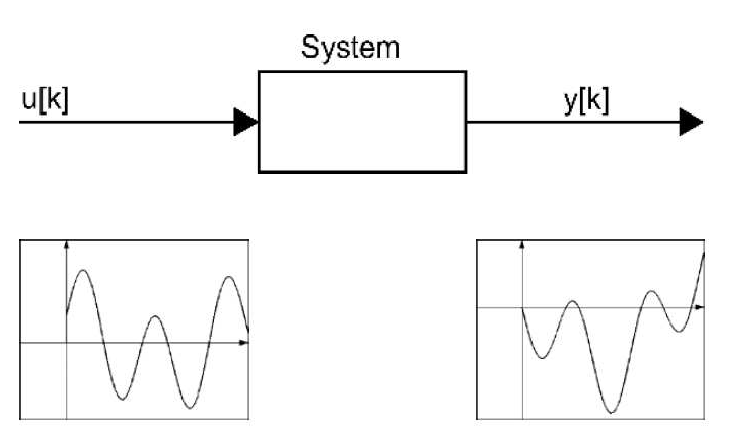
\includegraphics[width=0.8\linewidth]{continuous}
\end{figure}

\column{.5\textwidth}
\center {\textbf{Discrete}}\\
For every time step $k \in \mathds{Z}$, the system has: 
\begin{enumerate}
\item A vector of inputs \textbf{u}[k]
\item A vector of outputs \textbf{y}[k]
\item A vector of states \textbf{x}[k]
\end{enumerate}
\begin{figure}
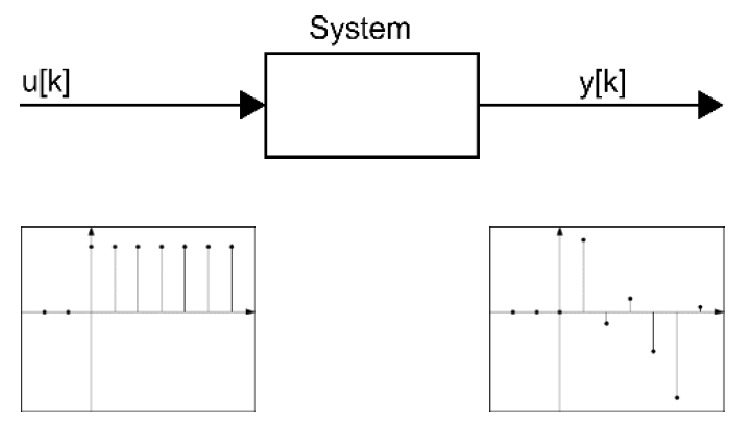
\includegraphics[width=0.8\linewidth]{discrete}
\end{figure}

\end{columns}
\end{frame}

%------------------------------------------------
\section{Linear vs. Nonlinear}
%------------------------------------------------

\begin{frame}
\frametitle{Linear vs. Nonlinear: a linear system}
\vspace{-2ex}
\textbf{Definition}\\
\medskip
A system is linear if \\
$\qquad u_{1}(t) \rightarrow y_{1}(t)\> \qquad \qquad (input\> u_{1}(t) \>results\> in\>output \>y_{1}(t))$\\
$\qquad u_{2}(t) \rightarrow y_{2}(t)$ \\
imply that \\
\vspace{-2ex}
\center{$\alpha u_{1}(t) + \beta u_{2}(t) \rightarrow \alpha y_{1}(t) + \beta y_{2}(t)$}\\
\bigskip
\begin{flushleft}
Properties of a linear system (contained in the definition):
\end{flushleft}
\vspace{-2ex}
\begin{itemize}
\item Superposition
\item Homogeneity
\end{itemize}
\end{frame}

%------------------------------------------------

\begin{frame}
\frametitle{Linear vs. Nonlinear: a linear system}
\textbf{Properties of a linear system} (contained in the definition):
\begin{itemize}
\item Superposition\\
\smallskip
\begin{center}
$u_{a}(t) \rightarrow y_{a}(t) \>\> and \>\> u_{b}(t) \rightarrow y_{b}(t)$\\
$ \Updownarrow$\\
$ u_{a}(t) + u_{b}(t) \rightarrow y_{a}(t) + y_{b}(t)$\\
\end{center}
\medskip
\small{This means the output produced by simultaneous applications of two different inputs is the sum of the two individual outputs.}
\item Homogeneity\\
\smallskip
$\alpha u(t) \rightarrow \alpha y(t)$\\
\end{itemize}
\smallskip
How to recognize a linear system:
\begin{itemize}
\item \small{Linear in all of the variables}
\item \small{No constant factors}
\end{itemize}
\end{frame}

%------------------------------------------------

\begin{frame}
\frametitle{Linear vs. Nonlinear: a linear system}
\textbf{Example}
\begin{align*}
\begin{cases} 
\dot{x} = u\\ 
\dot{y} = x + 2u
\end{cases}
\end{align*}
Linearity of this system is easily verified, based on the linearity of the derivative:\\
\vspace{-2ex}
\begin{align*}
\begin{cases} 
\textcolor{green}{\alpha \dot{x}_{a}(t)} + \textcolor{blue}{\beta \dot{x}_{b}(t)} = \textcolor{green}{\alpha u_{a}(t)} + \textcolor{blue}{\beta u_{b}(t)}\\ 
\textcolor{green}{\alpha \dot{y}_{a}(t)} + \textcolor{blue}{\beta \dot{y}_{b}(t}) = \textcolor{green}{\alpha x_{a}(t)} + \textcolor{blue}{\beta x_{b}(t)} + \textcolor{green}{2 \alpha u_{a}(t)} + \textcolor{blue}{2 \beta u_{b} (t)}
\end{cases}
\end{align*}
\end{frame}

%------------------------------------------------

\begin{frame}
\frametitle{Linear vs. Nonlinear: autonomous linear systems}
Continuous-time autonomous linear dynamical systems are described by:\\
\smallskip
\center{$\dot{x}(t) = Ax(t)$}\\
\begin{columns}
\column{.5\textwidth}
Example: $\dot{x}(t) = \begin{bmatrix} -1 & 0 \\ 2 & 1 \end{bmatrix} x(t)$

\column{.5\textwidth}
\begin{figure}
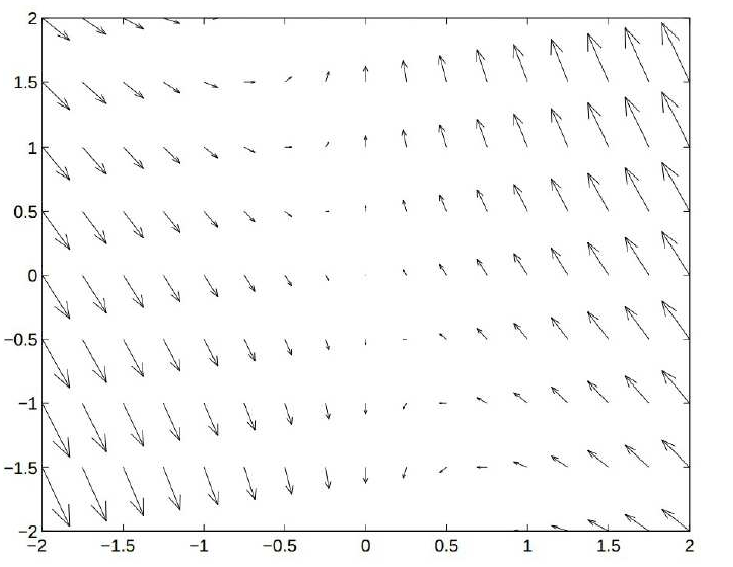
\includegraphics[width=1\linewidth]{autonomous}
\end{figure}
\end{columns}
\end{frame}

%------------------------------------------------

\begin{frame}
\frametitle{Linear vs. Nonlinear: violating homogeneity}
All nonhomogeneous systems are strictly speaking nonlinear, e.g.:\\
\begin{align*}
& \begin{cases}
\dot{x}(t) = x(t) + u(t)^{2}\\
\dot{y}(t) = x(t)
\end{cases} &&\text{$\Rightarrow$ nonhomogeneous}
\end{align*}

This is nonlinear, because the term $u(t)^{2}$ violates homogeneity.\\
It can be turned into a linear system with inputs $z(t) = u(t)^{2}$.

\begin{align*}
& \begin{cases}
\dot{x}(t) = x(t) + z(t)\\ 
\dot{y}(t) = x(t)
\end{cases} &&\text{$\Rightarrow$ linear}
\end{align*}
$\rightarrow$ nonhomogeneous systems that are linear apart from some function of inputs are often treated as linear systems.
\end{frame}

%------------------------------------------------

\begin{frame}
\frametitle{Linear vs. Nonlinear: nonlinear systems}
Some examples of nonlinear systems:
\begin{align*}
\begin{cases}
\dot{x}_{1}(t) = x_{1}(t) + u(t)\\
\dot{x}_{2}(t) = x_{1}(t) x_{2}(t)\\
y(t) = x_{1}(t) + x_{2}(t)
\end{cases}
\end{align*}

\begin{align*}
\begin{cases}
\dot{x}(t) = sin(x(t)) + u(t)\\
y(t) = x(t)
\end{cases}
\end{align*}

\begin{align*}
\begin{cases}
\dot{x}(t) = 2 u(t) + 1\\
y(t) = cos(x(t))
\end{cases}
\end{align*}

\end{frame}

%------------------------------------------------

\begin{frame}
\frametitle{Linear vs. Nonlinear systems}
\vspace{-8ex}
\begin{columns}
\column{.5\textwidth}
\textbf{\Large{Predominantly linear}}\\
\medskip
Simple electrical systems
\begin{itemize}
\item Circuits with ideal resistors, capacitors and inductors
\end{itemize}
Simple mechanical systems
\begin{itemize}
\item Systems with ideal springs
\end{itemize}
\bigskip

\column{.45\textwidth}
\textbf{\Large{Inherently nonlinear}}\\
\medskip
Chemical systems\\
\smallskip
Biological systems\\
\smallskip
Economical systems\\
\smallskip
More involved electrical or mechanical systems\\
\smallskip
...
\end{columns}
\end{frame}

%------------------------------------------------

\begin{frame}
\frametitle{Linear vs. Nonlinear systems}
\vspace{-6ex}
\begin{itemize}
\item Reality is nonlinear
\item However, this course will only deal with linear systems
\item Why do we prefer linear systems? \\
\medskip
The previously mentioned properties will allow for a thorough study of the system
\item Why are we allowed to use linear systems, even in a nonlinear setting?\\
\medskip
You can linearize around an equilibrium point (we will do this in the next lecture)
\end{itemize}
\end{frame}

%------------------------------------------------
\section{Causal vs. Non-causal} 
%------------------------------------------------

\begin{frame}
\frametitle{Causal vs. Non-causal systems}
\begin{itemize}
\item \normalsize{A causal system only depends on the present and the past, not on the future}
\item \normalsize{A non-causal system (also) depends on the future}
\item \normalsize{All physical systems are causal}
\begin{itemize}
\item \normalsize{A telephone:}
\begin{itemize}
\item \normalsize{It will not ring for future calls}
\end{itemize}
\item \normalsize{Any human:} 
\begin{itemize}
\item \normalsize{Is a system that will only react on inputs it has already received}
\item \normalsize{If we react because we expect something to happen in the future, then that expectation arose from past or present inputs}
\end{itemize}
\end{itemize}
\end{itemize}
\bigskip
\footnotesize{source: http://www.deekshith.in/2013/03/causal-and-non-causal-systems-better-explained.html}
\end{frame}

%------------------------------------------------

\begin{frame}
\frametitle{Causal vs. Non-causal systems}
\textbf{How do non-causal systems arise?}\\
\medskip
A possibility is by greatly reducing the complexity of a system, in which some causes of events are taken out of the equations.\\
Example:\\
\begin{itemize}
\small{
\item A model of the economical consumption (\textbf{output})
\item A lot of influencing factors, but the only \textbf{input} is the employment numbers
\item Current and past employment numbers determine consumption, but when someone gets fired, they will continue to work for several weeks in most instances, but their consumption will drop immediately
$\rightarrow$ A correct model would have to be \textbf{non-causal}
\item The non-causal model for this input-output relation is not useful if you want to determine the level of consumption
\item You could use the relation to see a drop in employment, before it is visible in the employment numbers}
\end{itemize}
\end{frame}

%------------------------------------------------

\begin{frame}
\frametitle{Causal vs. Non-causal systems}
Example of non-causal systems: \textbf{image processing}\\
\begin{itemize}
\small{
\item The input to our system (the image processor) is a two dimensional series of values ($u(k,l)$): the color values at the different pixels of the original image
\item The output is a processed image ($y(k,l)$)
\item There is now no reason to want causality; the input depends on position and not on time
\item $y(k,l)$ can rely on 'later' values like $u(k+1,l+1)$, without that being a problem}
\end{itemize}
\vspace{-2ex}
\begin{columns}
\column{.3\textwidth}
\begin{figure}
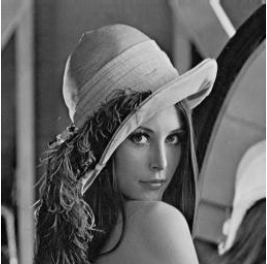
\includegraphics[width=.5\linewidth]{original}
\end{figure}
\vspace{-4ex}
\center{\small{Original image}}

\column{.3\textwidth}
\begin{figure}
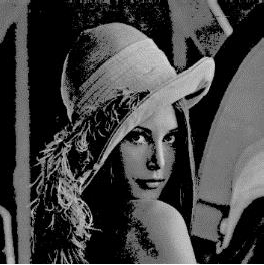
\includegraphics[width=.5\linewidth]{removed}
\end{figure}
\vspace{-4ex}
\center{\small{Removed details}}

\column{.3\textwidth}
\begin{figure}
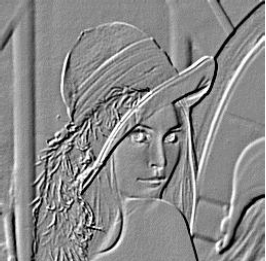
\includegraphics[width=.5\linewidth]{highlight}
\end{figure}
\vspace{-4ex}
\center{\small{Highlight borders}}

\end{columns}
\end{frame}

%------------------------------------------------

\begin{frame}
\frametitle{Causal vs. Non-causal systems}
\vspace{-6ex}
Some mathematical examples:\\
\bigskip
\begin{columns}
\column{.5\textwidth}
\textbf{Causal systems}\\
\begin{itemize}
\item \begin{align*}
\begin{cases}
x[k+1] = u[k]\\
y[k] = 3 x [k+1] + u[k]
\end{cases}
\end{align*}
\item $y(t) = 2 u(t-\tau)$
\end{itemize}

\column{.5\textwidth}
\textbf{Non-causal systems}\\
\begin{itemize}
\item \begin{align*}
\begin{cases}
x[k+1] = u[k])\\
y[k] = x[k+2] + \frac{1}{2}u[k]
\end{cases}
\end{align*}
\item $y(t) = u(t + \tau)$
\end{itemize}

\end{columns}
\end{frame}

%------------------------------------------------
\section{Time-invariant vs. Time-varying} 
%------------------------------------------------

\begin{frame}
\frametitle{Time-invariant vs. Time-varying systems}
Dynamics and properties of the system don't change through time.\\
If the same input is applied to a system that is in the same state, then the output of a time-invariant system will be the same.\\
\bigskip
Mathematically this looks as follows:\\
\begin{itemize}
\item In a time-invariant system:\\
if $u(t) \xrightarrow{x(t)} y(t)$ then $u(t+\tau) \xrightarrow{x(t+\tau)} y(t+\tau)$
\medskip
\item In time-varying systems, the parameters of the system are functions of time, e.g.:\\
\vspace{-2ex}
\begin{equation*}
\begin{cases}
             \dot{x}(t) = \textbf{A}x(t) + \textbf{B}u(t)\\
             y(t) = \textbf{C}x(t) + \textbf{D}u(t)
       \end{cases} \quad
\Rightarrow \quad
\begin{cases}
            \dot{x}(t) = \textbf{A}(t)x(t) + \textbf{B}(t)u(t)\\
             y(t) = \textbf{C}(t)x(t) + \textbf{D}(t)u(t)
       \end{cases}
\end{equation*}
\end{itemize}
\end{frame}

%------------------------------------------------

\begin{frame}
\frametitle{Time-invariant vs. Time-varying systems}
\textbf{Time-invariant differential equation}\\
\medskip
The dependent variable and its derivatives appear as linear combinations. The coefficients of all terms are constant.\\
Example: $\frac{d^{2}x}{dt^{2}} + 5\frac{dx}{dt} + 10x=0$\\
\bigskip
\bigskip
\textbf{Time-varying differential equation}\\
\medskip
The dependent variable and its derivatives appear as linear combinations, but coefficients of terms may involve the independent variable.\\
Example: $\frac{d^{2}x}{dt^{2}} + (1-cos(2t)x = 0$
\end{frame}

%------------------------------------------------

\begin{frame}
\frametitle{Time-invariant vs. Time-varying systems}
\begin{itemize}
\item Examples of time-varying systems:
\smallskip
\begin{itemize}
\item \normalsize{The properties of an electrical circuit slowly change over time}
\smallskip
\item \normalsize{The human body also has many changing properties}
\smallskip
\item \normalsize{Systems affected by night and day (heating of buildings), when those aspects were ignored in the model}
\end{itemize}
\medskip
\item Examples of time-invariant systems:
\smallskip
\begin{itemize}
\item \normalsize{A system that describes a physical law, for instance a system with two masses as its input and their attractive force as an output}
\smallskip
\item \normalsize{In practice we approximate all systems whose properties change much slower than the variables as time-invariant}
\end{itemize}
\end{itemize}
\end{frame}

%------------------------------------------------
\section{Lumped vs. Distributed parameter} 
%------------------------------------------------

\begin{frame}
\frametitle{Lumped vs. Distributed parameter systems}
Many physical phenomena are described mathematically by partial differential equations (PDEs). Such systems are called distributed parameter systems.\\
Lumped parameter systems are systems which can be described by ordinary differential equations (ODEs).\\
Example:\\
\begin{itemize}
\item Diffusion equation (discretize in space)
\item Heat equation
\end{itemize}
This means we need an \textbf{infinite amount of states}, we say that this is a \textbf{distributed system}.\\
If we have a \textbf{finite amount of states} (for instance by discretizing), we call the system a \textbf{lumped system}.\\
\end{frame}

%----------------------------------------------------------------------------------------

\end{document} 